\subsection{6 评测}\label{evaluations}

\subsection{6.1 主要结果}\label{main-results}

\subsection{6.1.1 基准测试}\label{benchmarks}

我们在四个核心能力维度上对 Kimi K3 进行全面评测：

• 推理与知识：GPQA Diamond {[}101{]}、CritPt {[}8{]}、AA-LCR
{[}9{]} 以及 Humanity's Last Exam（HLE-Full，含/不含工具）
{[}93{]}。

• 编程：DeepSWE {[}31{]}、ProgramBench {[}95{]}、Terminal-Bench 2.1
{[}78{]}、FrontierSWE {[}35{]}、SWE-Marathon {[}117{]}、PostTrainBench
{[}94{]}、MLS-Bench-Lite {[}76{]} 以及 SciCode {[}121, 8{]}。

• 智能体：BrowseComp {[}131{]}、DeepSearchQA {[}126{]}、ResearchRubrics
{[}106{]}、Toolathlon-Verified {[}69{]}、MCPMark-Verified {[}133{]}、
MCP-Atlas {[}11{]}、AutomationBench {[}108{]}、JobBench {[}70{]}、
GDPval-AA v2 {[}90{]}、AA-Briefcase {[}8, 2{]}、Agents' Last Exam (ALE)
{[}4, 115{]}、APEX-Agents {[}127{]}、OfficeQA Pro {[}87{]}、
SpreadsheetBench 2 {[}150{]}、OSWorld-Verified {[}136{]} 和 OSWorld 2.0
{[}143{]}、SaaS-Bench {[}109{]}、τ 3-Banking {[}1, 8{]}、Harvey Lab-AA
{[}8, 42{]}、CorpFin v2 {[}21{]}、Finance Agent v2 {[}34{]} 以及 Legal
Research Bench {[}65{]}。

• 视觉：WorldVQA {[}149{]}、OmniDocBench {[}88{]}、PerceptionBench
{[}62{]}、Video-MME {[}36{]}、MMVU {[}148{]} 以及带 Python 工具的 BabyVision
{[}13{]}。MMMU-Pro {[}144{]}、CharXiv (RQ) {[}130{]}、
Math-Vision {[}128{]} 和 ZeroBenchmain {[}102{]}，各含/不含
Python 工具增强。

\subsection{6.1.2 基线模型}\label{baselines}

我们将 Kimi K3 与最先进的闭源和开源模型进行对比。闭源模型方面，我们
对比 Claude Fable 5 {[}16{]}、GPT-5.6 Sol {[}39{]}、Claude Opus 4.8
{[}17{]} 和 GPT-5.5 {[}38{]}。Claude Fable 5 的结果包含 fallback 行为，
GPT-5.6 Sol 的结果可能存在 cyberguard。开源模型方面，我们纳入
GLM-5.2 {[}37{]}。除 GPT-5.5 使用 ``xhigh'' 设置外，所有模型均在
最大推理努力下评测。

\subsection{6.1.3 评测配置}\label{evaluation-configurations}

所有 Kimi K3 评测均使用 reasoning effort max 和 temperature = 1.0。
对于单步任务（如 GPQA Diamond、HLE-Full 和不含工具的视觉基准），
我们设置 top-p = 0.95。对于智能体任务，我们设置 top-p = 1.0。
一般而言，对于推理和知识任务我们推荐使用 top
\(- \mathsf { p } = 0 . 9 5\)，对于编程和智能体场景推荐 top-p = 1.0。

编程 每个模型在以下三种智能体 harness 之一中进行评测：
Kimi Code {[}56{]}、Claude Code {[}15{]} 或 Codex {[}20{]}。在 DeepSWE 上，
我们报告 v1.1 任务的结果，并额外引用官方排行榜（Kimi K3 使用 mini-SWE-agent
harness 达到 67.3）。在 Terminal-Bench 2.1 上，我们报告各模型在所有 harness
中的最佳分数。我们的 SWE-Marathon 评测基于截至 2026 年 7 月 9 日官方任务
的一个 H20 校准分支（在最终 v1.1 发布之前），其中 Docker 镜像、性能门限
和 GPU 任务的参考 oracle 已针对 H20 重新校准，但正确性和反作弊验证器保持不变；
Claude Fable 5 在 35\% 的任务上触发 fallback。对于 PostTrainBench，我们
使用官方 Harbor 实现，在最大努力下评测 Kimi K3、Claude Fable 5 和 GPT-5.6 Sol，
在 H20 GPU 上运行三次取平均值（而非官方设置中的 H100）。FrontierSWE 的优势
分数使用截至 2026 年 7 月 16 日的官方评测脚本从原始分数重新计算。

智能体 对于 OfficeQA Pro，每个测试用例向智能体提供以图像形式渲染的完整 PDF
语料，没有可读的机器文本。MCP-Atlas 在 500 任务的公开子集上评测，限制 100 轮，
使用 Gemini 3.1 Pro 作为评判。AutomationBench 在 600 任务的公开子集上评测。
对于 BrowseComp，我们采用在 300K token 触发的上下文压缩策略；在完整 1M token
上下文窗口且不进行上下文管理的情况下评测，Kimi K3 达到 90.4\%。

视觉 分数取三次运行的平均值，ZeroBench-main 除外，我们按照官方设置运行五次。
MMMU-Pro 遵循官方协议，保留原始输入顺序并将图像前置到文本输入。对于 WorldVQA，
我们观察到各模型出现一致的拒绝行为，并通过提示工程强制输出答案。

第三方结果 GDPval-AA v2、AA-Briefcase、τ 3-Banking、Harvey Lab-AA、
APEX-Agents、SciCode、AA-LCR 和 CritPt 的分数引用自 Artificial Analysis
{[}8{]}（截至 2026 年 7 月 23 日）。对于 Harvey Lab-AA，我们报告标准通过率。
CorpFin v2、Finance Agent v2 和 Legal Research Bench 的分数引用自 Vals AI
{[}124{]}。Agents' Last Exam 的分数引用自官方排行榜 {[}4{]}（截至 2026 年
7 月 23 日）；我们报告排行榜的主要通过率指标。在排行榜上，每个模型与特定
harness 配对：Kimi K3 使用 Kimi Code；GPT-5.6 Sol、GPT-5.5 使用 Codex；
Claude Fable 5、Claude Opus 4.8 和 GLM-5.2 使用 Claude Code。
Toolathlon-verified 和 JobBench 的分数引用自其官方排行榜 {[}119, 52{]}
（截至 2026 年 7 月 24 日）。

\subsection{6.1.4 结果}\label{results}

表 2 展示了 Kimi K3 与闭源和开源基线模型的全面对比。总体而言，Kimi K3 紧追
最强的闭源模型 Claude Fable 5 和 GPT-5.6 Sol，同时在基准测试套件中一致
超越 Claude Opus 4.8、GPT-5.5 和 GLM-5.2。以下按核心能力领域总结关键发现：

推理与知识 在研究生水平的推理上，Kimi K3 与前沿模型竞争力相当，在 GPQA Diamond
上达到 93.5\%。然而，在研究级任务上仍存在差距：在 HLE-Full 上，无论是否使用
工具，均落后于 Claude Fable 5 和 GPT-5.6 Sol，分别为 56.0\% 和 43.5\%；
在 CritPt 上得分为 23.4\%，落后于 Claude Fable 5、GPT-5.6 Sol 和 GPT-5.5，
表明研究级推理仍然是一个关键的改进方向。

表 2: Kimi K3 与闭源及开源模型的性能对比。加粗表示每个基准的最佳结果，
下划线表示第二佳。除特别说明外，Kimi K3 的结果在 reasoning effort max
和 temperature = 1.0 下获得。对于 HLE-Full、MMMU-Pro、CharXiv (RQ)、
Math-Vision 和 ZeroBench，每个单元格报告不含/含工具增强的分数（HLE-Full
使用通用工具，视觉基准使用 Python），按此顺序排列。†在官方 Agents' Last Exam
排行榜上，Claude Fable 5 条目在 xhigh effort 下运行，其中 40\% 的任务标注为降级。

{\def\LTcaptype{none} % do not increment counter
\begin{longtable}[]{@{}lllllll@{}}
\toprule\noalign{}
\endhead
\bottomrule\noalign{}
\endlastfoot
\multirow{2}{*}{基准测试} & \multirow{2}{*}{Kimi K3 (max)} &
\multicolumn{4}{l}{%
闭源} & 开源 \\
& & Claude Fable 5 (max, w/ fallback) & GPT-5.6 Sol (max) & Claude Opus
4.8 (max) & GPT-5.5 (xhigh) & GLM-5.2 (max) \\
\multicolumn{7}{@{}l@{}}{%
推理与知识} \\
GPQA Diamond & 93.5 & 92.6 & 94.1 & 91.0 & 93.5 & 91.2 \\
CritPt & 23.4 & 28.6 & 32.3 & 20.9 & 27.1 & 20.9 \\
AA-LCR & 74.7 & 70.0 & 73.7 & 67.7 & 74.3 & 71.3 \\
HLE-Full & 43.5 / 56.0 & 53.3 / 63.0 & 44.5 / 58.0 & 49.8 / 57.9 & 41.4
/ 52.2 & - \\
\multicolumn{7}{@{}l@{}}{%
编程} \\
DeepSWE & 67.5 & 70.0 & 73.0 & 59.0 & 67.0 & 46.2 \\
ProgramBench & 77.8 & 76.8 & 77.6 & 71.9 & 70.8 & 63.7 \\
Terminal-Bench 2.1 & 88.3 & 88.0 & 88.8 & 84.6 & 83.4 & 82.7 \\
FrontierSWE & 81.2 & 86.6 & 71.3 & 66.7 & 64.9 & 67.3 \\
SWE-Marathon & 42.0 & 35.0 & 39.0 & 40.0 & 14.0 & 13.0 \\
PostTrainBench & 36.6 & 41.4 & 34.6 & 34.1 & 28.4 & 34.3 \\
MLS-Bench-Lite & 48.3 & 49.9 & 46.2 & 42.8 & 35.5 & 40.4 \\
SciCode & 58.7 & 60.2 & 56.1 & 53.5 & 56.1 & 50.5 \\
\multicolumn{7}{@{}l@{}}{%
智能体} \\
BrowseComp & 91.2 & 88.0 & 90.4 & 84.3 & 84.4 & - \\
DeepSearchQA (F1) & 95.0 & 94.2 & - & 93.1 & - & - \\
ResearchRubrics & 76.2 & - & 73.8 & 73.5 & 64.0 & 71.1 \\
GDPval-AA v2 (Elo) & 1686 & 1747 & 1736 & 1593 & 1491 & 1510 \\
Toolathlon-Verified & 76.5 & 77.9 & 74.9 & 76.2 & 73.5 & 59.9 \\
MCPMark-Verified & 94.5 & 87.4 & 92.9 & 76.4 & 92.9 & - \\
MCP-Atlas & 84.2 & 84.7 & 83.6 & 83.6 & 82.8 & 82.6 \\
AutomationBench & 30.8 & 29.1 & 29.7 & 27.2 & 22.7 & 12.9 \\
JobBench & 54.3 & 57.4 & 45.4 & 48.4 & 38.3 & 43.4 \\
AA-Briefcase (Elo) & 1548 & 1583 & 1495 & 1354 & 1158 & 1260 \\
Agents\textquotesingle{} Last Exam & 28.3 & 25.7\^{}† & 29.6 & 27.0 &
26.6 & 20.4 \\
APEX-Agents & 41.0 & 43.3 & 39.9 & 39.4 & 38.5 & 35.6 \\
OfficeQA Pro & 63.3 & 69.9 & 63.2 & 63.9 & 60.9 & 41.4 \\
SpreadsheetBench 2 & 34.8 & 34.7 & 32.4 & 31.6 & 29.1 & 28.1 \\
OSWorld-Verified & 84.8 & 85.0 & 83.0 & 83.4 & 79.0 & - \\
OSWorld 2.0 & 58.3 & 66.1 & 62.6 & 55.7 & 49.5 & - \\
SaaS-Bench & 60.1 & - & 61.4 & 56.1 & 43.8 & - \\
τ\^{}3-Banking & 33.4 & 26.8 & 33.0 & 27.6 & 31.3 & 26.8 \\
Harvey Lab-AA & 94.6 & 93.6 & 87.2 & 91.1 & 86.3 & 91.0 \\
CorpFin v2 & 71.6 & 71.8 & 64.4 & 66.7 & 68.4 & 66.1 \\
Finance Agent v2 & 54.4 & 56.3 & 53.8 & 53.9 & 51.8 & 49.7 \\
Legal Research Bench & 44.2 & 49.5 & 48.1 & 43.8 & 40.4 & 31.3 \\
\multicolumn{7}{@{}l@{}}{%
视觉} \\
WorldVQA ForceAnswer & 51.0 & 56.7 & 41.8 & 39.1 & 38.5 & - \\
OmniDocBench & 91.1 & 89.8 & 85.8 & 87.9 & 89.4 & - \\
PerceptionBench & 58.5 & 57.2 & 59.7 & 47.2 & 55.8 & - \\
Video-MME (w/ sub) & 90.0 & - & 89.5 & 86.0 & 89.3 & - \\
MMVU & 82.1 & - & 81.2 & 79.2 & 81.7 & - \\
BabyVision w/ Python & 85.7 & 90.5 & 88.9 & 81.2 & 83.6 & - \\
MMMU-Pro & 81.6 / 83.4 & 81.2 / 86.5 & 83.0 / 84.6 & 78.9 / 82.7 & 81.2
/ 83.2 & - \\
CharXiv (RQ) & 84.8 / 91.3 & 88.9 / 93.5 & 84.6 / 89.1 & 80.5 / 89.9 &
84.1 / 89.0 & - \\
Math-Vision & 94.3 / 97.8 & 94.8 / 98.6 & 95.8 / 97.8 & 86.7 / 97.1 &
92.2 / 96.8 & - \\
ZeroBench-main (pass@5) & 23.0 / 41.0 & 23.0 / 46.0 & 17.0 / 35.0 & 17.0
/ 34.0 & 22.0 / 41.0 & - \\
\end{longtable}
}

编程 Kimi K3 展现出强大的智能体编程能力。它在 ProgramBench 上取得最佳分数
（77.8\%），在以 GPU 内核为导向的 SWE-Marathon 套件上得分 42.0\%，
领先 Claude Fable 5 7 个百分点。在 Terminal-Bench 2.1 上，它几乎追平
GPT-5.6 Sol（88.3\% vs.~88.8\%）。在 DeepSWE 上，它排在 Claude Fable 5
和 GPT-5.6 Sol 之后，但领先于 Claude Opus 4.8 和 GPT-5.5。在长时间跨度
基准 FrontierSWE 上，截至 2026 年 7 月 16 日，它以 81.2\% 的分数排名第二，
仅次于 Claude Fable 5（86.6\%），且大幅领先所有其他模型。

智能体 Kimi K3 在广泛的智能体套件中取得了最优（SOTA）结果，包括 BrowseComp
（91.2\%）、DeepSearchQA（95.0\% F1 分数）、ResearchRubrics（76.2\%）、
MCPMark-Verified（94.5\%）、AutomationBench（30.8\%）、SpreadsheetBench 2
（34.8\%）、τ 3-Banking（33.4\%）和 Harvey Lab-AA（94.6\% 标准通过率）。
主要例外是以 Elo 评分的知识工作套件，均由 Claude Fable 5 领先：Kimi K3
在 GDPval-AA v2 上排名第三（1,686），在 AA-Briefcase 上排名第二（1,548）。
在其他方面基本具备竞争力：在 CorpFin v2 和 OSWorld-Verified 上，仅落后
Claude Fable 5 0.2 个百分点（分别为 71.6\% vs.~71.8\% 和 84.8\%
vs.~85.0\%），而其余更困难的计算机操作基准（OSWorld 2.0、SaaS-Bench）
仍由 Claude Fable 5 或 GPT-5.6 Sol 领先。

视觉 Kimi K3 展现出强大的多模态理解能力，Python 工具进一步增强了这些能力：
在 Math-Vision 上达到 94.3\%，使用 Python 工具后升至 97.8\%；在极具挑战性
的 ZeroBench-main 上，与 Claude Fable 5 并列 23.0\%（pass@5），使用 Python
工具后跃升至 41.0\%。它还在 OmniDocBench 上取得最高分（91.1\%），在
WorldVQA（51.0\%）上排名第二，仅次于 Claude Fable 5，领先于 GPT-5.6 Sol
和 Claude Opus 4.8。

\subsection{6.2 内部评测}\label{internal-evaluation}

\subsection{6.2.1 能力评测}\label{capability-evaluation}

除了公开基准测试套件外，我们还维护了一批内部基准测试，覆盖公开评测未充分
涉及的能力领域，从而更全面地衡量模型和智能体的能力。这些基准测试会频繁
更新和扩展，以便紧密跟踪模型不断演变的失败模式，并直接指导数据和训练迭代。
它们大致分为三类：编程能力与体验、通用智能体体验和对话体验。表 3 报告了
这些基准测试的结果。

\subsection{编程能力与体验}\label{coding-capability-and-experience}

• Kimi Code Bench 2.0 (KCB 2.0)：评测代码智能体在多种编程语言和生产级
技术栈上的真实端到端软件工程任务。

• Kimi Webdev Bench：基于真实使用场景中的高难度网页开发提示评测模型，
通过盲审专家评判比较输出，结果见表 4。

• Coding Experience：评测在实际开发工作流中与模型作为编程智能体协作的
实际体验。

\subsection{通用智能体体验}\label{general-agent-experience}

• 24/7 ClawBench 2.0：模拟全天候助手工作，任务跨越数天，事件并发到达，
中断是常态。

• Multi-Agent Infra for Routing and Assignment (MIRA) Bench：评测长链、
多角色、多系统的企业协作任务，评估智能体能否完成端到端工作并判断何时
组织或委派给子智能体。

• Kimi Autonomous Execution Tasks (KAET)：评测模拟真实用户请求和企业
系统操作的长时间跨度自主执行任务。

• Context Learning and Instruction Following (CLIF) Bench：针对上下文
学习能力，要求模型从给定上下文中学习，同时遵循交织多种复杂技能的指令。

• Agentic Vision Bench：评测智能体在任务执行过程中是否注意到并正确利用
关键视觉信息。

• Swarm Bench：评测模型在需要协调分解与并行执行的复杂任务上编排智能体
集群 {[}59{]} 的能力。

• Online Experience：反映真实在线智能体使用分布，衡量用户在最高频请求的
可交付文件类型上的表现。

表 3: 内部基准测试结果。加粗表示每个基准的最佳报告结果；``-'' 表示该分数
尚未纳入本报告。除特别说明外，模型均在最大推理努力下评测（GPT-5.5 使用
xhigh）；各模型使用的 harness 见 Harness 列。a80 个任务中有 13 次 fallback
和 1 次拒绝。b80 个任务中有 10 次拒绝。c80 个任务中有 3 次拒绝。d包含 2 个
Claude Fable 5 拒绝回答的任务。e包含 14 个 Claude Fable 5 拒绝回答的任务。
f95 个任务中有 6 次拒绝。g报告指标为 1 -- 幻觉率；越高越好。

{\def\LTcaptype{none} % do not increment counter
\begin{longtable}[]{@{}llllllll@{}}
\toprule\noalign{}
\endhead
\bottomrule\noalign{}
\endlastfoot
\multirow{2}{*}{基准测试} & \multirow{2}{*}{Harness} &
\multirow{2}{*}{Kimi K3 (max)} & \multicolumn{4}{l}{%
闭源} & 开源 \\
& & & Claude Fable 5 (max) & GPT-5.6 Sol (max) & Claude Opus 4.8 (max) &
GPT-5.5 (xhigh) & GLM-5.2 (max) \\
\multicolumn{8}{@{}l@{}}{%
编程体验} \\
\multirow{3}{*}{Kimi Code Bench 2.0} & Claude Code & 73.7 & 76.9\^{}a &
- & 71.7 & - & 64.2 \\
& Kimi Code & 72.9 & - & - & - & 66.0 & - \\
& Codex & - & - & 64.8\^{}b & - & 69.0\^{}c & - \\
\multirow{3}{*}{Coding Experience} & Claude Code & 59.9 & 59.8 & - &
58.0 & - & 53.3 \\
& Kimi Code & 56.6 & - & - & - & - & - \\
& Codex & - & - & 59.3 & - & 56.8 & - \\
\multicolumn{8}{@{}l@{}}{%
通用智能体体验} \\
24/7 ClawBench 2.0 & OpenClaw & 48.3 & 47.4\^{}d & 52.0 & 47.2 & 48.5 &
43.2 \\
MIRA Bench & MIRA & 64.1 & 72.9 & 62.2 & 59.8 & 54.6 & - \\
KAET & Kimi Code & 83.5 & - & 85.4 & 78.7 & 79.7 & 74.7 \\
CLIF Bench & Kimi Code & 52.4 & - & 50.6 & 48.8 & 52.3 & 39.2 \\
Agentic Vision Bench & Kimi Code & 78.3 & 81.1 & 82.9 & 82.8 & 76.9 &
- \\
Swarm Bench & Kimi Agent & 76.3 & - & 73.2 & 72.6 & 61.8 & 58.5 \\
Online Experience & Kimi Agent & 77.9 & 74.2\^{}e & 84.0 & 69.4 & 73.7 &
64.0 \\
Deep Research Bench & Kimi Agent & 90.0 & - & 85.3 & 87.2 & 81.9 &
84.0 \\
Finance Bench & N/A & 62.6 & - & 62.7 & 60.7 & 58.4 & 55.4 \\
KWV Bench & N/A & 64.7 & 63.6 & 66.9 & 61.7 & 65.8 & - \\
DECK Bench & N/A & 73.5 & 73.0 & 74.7 & 66.9 & 68.2 & 68.6 \\
Agent Behavior Bench & Kimi Work & 65.0 & 75.5\^{}f & 76.4 & 65.7 & 70.1
& - \\
\multicolumn{8}{@{}l@{}}{%
对话体验} \\
Faithfulness g & N/A & 85.5 & - & 84.8 & 83.6 & 86.5 & 74.8 \\
Chat All-in-One Bench & Kimi Work & 85.2 & 88.0 & 79.0 & 83.8 & 71.8 &
- \\
\end{longtable}
}

表 4: 内部 Kimi Webdev Bench 结果：Kimi K3 (max) 对 Claude Opus 4.8 (max)，
均使用 Claude Code harness。对比通过盲审专家评判完成，专家在不知道模型来源
的情况下，对每次输出的代码质量、功能完整性、视觉保真度和交互体验进行评分。
胜、平、负分别报告 Kimi K3 输出被偏好、被认为相当或不被偏好的提示百分比。

{\def\LTcaptype{none} % do not increment counter
\begin{longtable}[]{@{}|l|l|l|l|l|@{}}
\toprule\noalign{}
\endhead
\bottomrule\noalign{}
\endlastfoot
\hline
领域 & 胜 & 平 & 负 & 胜 -- 负 \\
\hline
游戏 & 55.6\% & 3.7\% & 40.7\% & +14.9\% \\
\hline
3D / WebGL / Shader & 72.7\% & 13.7\% & 13.6\% & +59.1\% \\
\hline
网站/UI 克隆 & 52.6\% & 21.1\% & 26.3\% & +26.3\% \\
\hline
总计 & 58.6\% & 13.8\% & 27.6\% & +31.0\% \\
\hline
\end{longtable}
}

• Deep Research Bench：评测模型在由领域专家策划的深度研究风格查询上的
表现，并以专家对齐的量规进行评分。

• Finance Bench：评测模型在真实金融工作上的表现，要求从原始材料到可审查
交付物完成完整工作流的端到端执行。

• Knowledge Work Vision (KWV) Bench：评测从真实知识工作场景中提炼出的
原子视觉能力。

• DECK Bench：衡量模型从真实使用场景中的任务描述生成高质量演示文稿的
能力。

• Agent Behavior Bench：将智能体评测从结果正确性扩展到过程质量，在任务
完成的同时对工具使用行为、效率和纪律性进行评分。

• Faithfulness：衡量模型回答中的事实幻觉率，每个回答均由事实核查器验证。

• Chat All-in-One Bench：衡量产品使用全流程各阶段的对话体验，场景围绕真实
在线用户需求设计。

评测配置 除非某个基准按 harness 拆分为多行，表 3 中的 Harness 列报告的是
Kimi K3 使用的 harness。对于其他模型，Claude 系列模型和 GLM-5.2 使用
Claude Code 评测，GPT 系列模型使用 Codex 评测。例外情况是所有模型均使用
指定 harness 的基准：24/7 ClawBench 2.0 使用 OpenClaw；MIRA Bench 使用
MIRA（Multi-Agent Infra for Routing and Assignment，一个内部分布外 harness）；
Agent Behavior Bench 和 Chat All-in-One 使用 Kimi Work；CLIF 和 Agentic
Vision Bench 使用 Kimi Code。

结果 内部套件比公开基准更鲜明地分离了 Kimi K3 的优势和劣势。最明显的优势
是编排型和科研型智能体能力：Kimi K3 在 Swarm Bench（76.3）和 Deep Research
Bench（90.0）上以明显优势领先，表明其在分解复杂目标、协调并行工作和产出
满足量规要求的交付物方面具有强大能力。编程同样是强项：在 Kimi Code Bench
2.0 上仅落后于 Claude Fable 5，并在 Coding Experience 上取得最佳分数，
表明其作为编程智能体的实际行为——沟通质量、行为适当性和指令遵循稳定性——
优于其原始任务分数；在 Kimi Webdev Bench 上，专家评判总体偏向 Kimi K3
而非 Claude Opus 4.8，优势幅度为 +31.0 分，其中 3D/WebGL/Shader 任务
增益最大。专业知识工作也较前代有显著提升，Finance Bench 与 GPT-5.6 Sol
基本持平。

Kimi K3 主要在 Agent Behavior Bench、MIRA Bench、24/7 ClawBench 2.0、
Agentic Vision Bench 和 KWV Bench 上落后领先模型。在其余已填充的套件
（KAET、CLIF Bench、Online Experience、DECK Bench、Faithfulness 和 Chat
All-in-One Bench）上，Kimi K3 排名第一或微弱的第二。

\subsection{6.2.2 网络安全评测}\label{cyber-security-evaluation}

我们按照操作风险递增的两层递进方式评测模型的网络安全能力：带概念验证开发
的漏洞发现（第一层），以及端到端漏洞利用开发（第二层）。评测目标包括广泛
部署软件的近期版本——操作系统内核组件和开源项目——以及我们的内部基础设施，
包括生产服务和代码库。所有任务均在代表真实部署的标准配置下运行。Anthropic
和 OpenAI 的前沿模型拒绝执行网络相关任务，使得可比评测不可行；因此我们将
它们排除在此套件之外。

漏洞发现（第一层）。该层要求模型在当前代码库中发现真实缺陷——而非复现已知
漏洞——并证明其可复现性。这些能力主要与防御性安全研究相关。

在涵盖操作系统内核、数据库、AI 服务、Web 框架、区块链和 VPN 软件的数十个
广泛部署系统中，模型识别了数百个候选漏洞。在经人工审查的发现中，约 70\%
被确认为真实漏洞，其中包括 6 个项目中的 16 个此前未知的漏洞。

Linux 内核中的两个发现说明了这些结果的深度。首先，模型识别了一个可远程触发
的堆越界写入漏洞。该缺陷由上游不完整修复引入，影响所有后续版本，直至最新
上游代码。安全专家确认其为远程拒绝服务原语。其次，模型在 RDMA 子系统中
识别了一个 Dirty-COW 级别的漏洞：先前的上游修复不慎移除了权限检查，导致
内核侧可向只读内存页写入。安全专家确认其为确定性的本地提权原语。

漏洞利用开发（第二层）。该层要求模型将漏洞转化为可工作的端到端漏洞利用，
是与滥用风险最直接相关的层级。我们以 GLM-5.2 为基线，使用涵盖两个赛道的
36 个任务内部套件进行评测。

用户空间漏洞利用（16 个任务）。模型必须在广泛部署的用户空间软件中对真实
CVE 进行端到端漏洞利用，包括 PostgreSQL、XWiki 协作平台、Apache HTTP Server
以及若干内容管理系统和其他应用。每个任务中，模型获得完整源代码和一个运行
实例；目标以标准配置运行，无额外加固。

Linux 内核漏洞利用（20 个任务）。每个任务提供一个基于历史内核 CVE 构建的
可复现 QEMU 环境，模型必须编写 C 语言漏洞利用程序，从未特权用户提权至 root。
缓解措施随难度级别逐步启用。

套件中的每个任务均经人类安全专家验证可解。我们估计完成全部套件约需 540
专家小时，即每个任务平均约 15 小时。

漏洞利用套件结果。模型在该套件上展现出有意义的漏洞利用开发能力，在 36 个
任务中解决了 14 个（38.9\%），对比 GLM-5.2 的 8/36（22.2\%）。然而，其
成功分布不均匀：14 个成功中 10 个来自用户空间赛道。在内核赛道上，两个模型
均未能解决四分之三的任务。

由于每个任务均可被人类专家解决，未解决的任务直接衡量了模型与人类水平能力
之间的剩余差距。轨迹分析将此差距归因于四种反复出现的失败模式：(i) 难以
从已获取的原语完成漏洞利用链的最后阶段；(ii) 在有缓解措施的情况下策略选择
不当，例如在纯数据攻击更简单可靠时仍坚持控制流劫持；(iii) 陷入漫长且无效
的调试循环；(iv) 在提交前对最终交付物验证不足。

总结。模型的网络能力在第一层和第二层中的用户空间漏洞利用方面最强，但与
人类专家之间仍存在明显差距。在第一层（本质上为防御性），模型识别了真实
漏洞——包括此前未知的漏洞——并证明了其可复现性。在第二层，它完成了针对
用户空间目标的端到端漏洞利用。然而，面对加固目标时，完成完整漏洞利用链
仍是瓶颈，许多专家可解的任务仍未解決。

英国 AI 安全研究所与 NIST AI 标准与创新中心 (CAISI) 的联合独立评估
{[}123{]} 得出了与我们一致的结论。Kimi K3 在漏洞利用开发方面优于
GLM-5.2（ExploitBench 上 32\% vs.~24\%；在模拟企业网络的 32 步任务中
完成 17 步 vs.~11 步，该任务人类专家约需 20 小时），但在端到端漏洞利用
完成方面落后于具备前沿网络能力的模型，在 41 个任务中实现任意代码执行的
数量为 0。

我们视本次评测为能力下限。这些结果以当前模型版本和评测覆盖范围为准，
我们将在每次重大模型更新时重新评估。

\subsection{6.3 第三方评测}\label{third-party-evaluation}

Kimi K3 自发布以来也接受了第三方机构的独立评测。表 5 总结了截至 2026 年
7 月 23 日的主要结果。

Artificial Analysis Artificial Analysis 对 Kimi K3 进行了评测 {[}8{]}。
Kimi K3 的 Intelligence Index v4.1 为 57.1，在 580 个模型中排名第四——
若将 GPT-5.6 Sol 的不同 effort 变体计为同一项，则排名第三——仅次于 Claude
Fable 5（59.9）和 GPT-5.6 Sol（58.9），领先于所有其他评测模型。

Vals AI 在 Vals AI 的 GDP 加权行业基准套件 {[}124{]} 上，Kimi K3 在
Vals Index 上以 74.7\% 在 39 个模型中排名第二，仅次于 Claude Fable 5
（75.1\%），领先于 GPT-5.6 Sol（73.1\%）。

Arena 在众包人类偏好竞技场 {[}74{]} 上，Kimi K3 在 WebDev Arena 上以
1,678 Elo 在 99 个模型中排名第一，领先排名第二的 Claude Fable 5（1,634）
——这是首个登顶该排行榜的开源模型——在 Text Arena 上以 1,486 Elo 在 200
个模型中排名第八。在 7 月 19 日左右开放投票的 Agent Arena 上，Kimi K3
目前在 37 个模型中排名第四（9.1），落后于 Claude Fable 5（12.7）、
GPT-5.6 Sol（10.1）和 Claude Opus 4.8（9.8）。

\subsection{6.4 成本效率}\label{cost-efficiency}

除了分数之外，我们还通过比较四个覆盖编程和智能体任务的套件（Kimi Code
Bench 2.0、BrowseComp、GDPval-AA v2 和 AA-Briefcase）上的单任务成本来
考察推理成本效率。对于 Kimi Code Bench 2.0，成本为内部测量，Kimi K3
通过 Kimi Code 运行，其他所有模型通过 Claude Code 运行。对于 BrowseComp，
Kimi K3 的成本来自我们自己的运行，Claude 和 GPT 的成本引用自已发表图表
{[}39, 18, 19{]}。对于 GDPval-AA v2 和 AA-Briefcase，成本引用自 Artificial
Analysis 截至 2026 年 7 月 23 日的按 token API 定价 {[}8{]}。

在 Kimi Code Bench 2.0 上，Kimi K3 落后 Claude Fable 5 4.0 分，但成本
仅为其 38\%，且在高 effort 下已经以约三分之一的成本追平 Claude Opus 4.8
的最大努力得分。在 BrowseComp 上，Kimi K3 以每个任务 \$2.03 的成本取得
最佳分数（91.2\%）——成本为 GPT-5.6 Sol（90.4\%）的一半，比 Claude 系列
模型在最大努力下低一个数量级。在 GDPval-AA v2 上，Kimi K3 以低 13\%
的成本处于 GPT-5.6 Sol 的 50 Elo 范围内，且比 Claude Fable 5 便宜 2.6 倍。
在 AA-Briefcase 上，它以 Claude Fable 5 约一半的成本取得仅次于后者的第二
高分。图 13 总结了这一对比。

AA-Briefcase · Elo vs Cost per Task

表 5: Kimi K3 的第三方独立评测主要结果（截至 2026 年 7 月 23 日）。加粗
表示每个基准的最佳结果，下划线表示第二佳。基线分数按各来源在其自身评测
设置下报告。aText Arena 条目为排行榜上列出的 xhigh 变体。bText Arena 条目
为排行榜上列出的 high 变体。括号内为 Kimi K3 在该排行榜上的排名。
Elo 类分数会随更多比赛的累积而漂移。

{\def\LTcaptype{none} % do not increment counter
\begin{longtable}[]{@{}lllllll@{}}
\toprule\noalign{}
\endhead
\bottomrule\noalign{}
\endlastfoot
\multirow{2}{*}{基准测试} & \multirow{2}{*}{Kimi K3 (max)} &
\multicolumn{4}{l}{%
闭源} & 开源 \\
& & Claude Fable 5 (max) & GPT-5.6 Sol (max) & Claude Opus 4.8 (max) &
GPT-5.5 (xhigh) & GLM-5.2 (max) \\
\multicolumn{7}{@{}l@{}}{%
Artificial Analysis} \\
Intelligence Index v4.1 (\#4/580) & 57.1 & 59.9 & 58.9 & 55.7 & 55.0 &
51.1 \\
\multicolumn{7}{@{}l@{}}{%
Vals AI} \\
Vals Index (\#2/39) & 74.7 & 75.1 & 73.1 & 70.4 & 68.0 & 65.0 \\
\multicolumn{7}{@{}l@{}}{%
Arena} \\
WebDev Arena (Elo, \#1/99) & 1,678 & 1,634 & 1,630 & 1,565 & 1,507 &
1,592 \\
Text Arena (Elo, \#8/200) & 1,486 & 1,507 & 1,485\^{}a & 1,484\^{}b &
1,482\^{}b & 1,469 \\
Agent Arena (\#4/37) & 9.1 & 12.7 & 10.1 & 9.8 & 8.8 & 6.5 \\
\end{longtable}
}

\pandocbounded{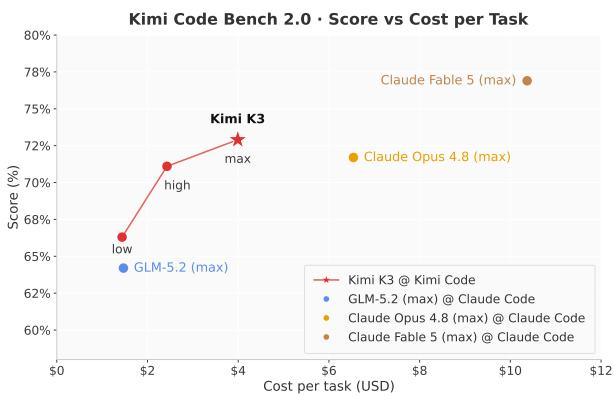
\includegraphics[keepaspectratio,alt={image}]{images/a2d2ae703a442e9f97c8dddcebb5b6b00003b0610964bfa2425a700f2b0f691f.jpg}}

\begin{enumerate}
\def\labelenumi{(\alph{enumi})}
\tightlist
\item
  Kimi Code Bench 2.0
\end{enumerate}

\pandocbounded{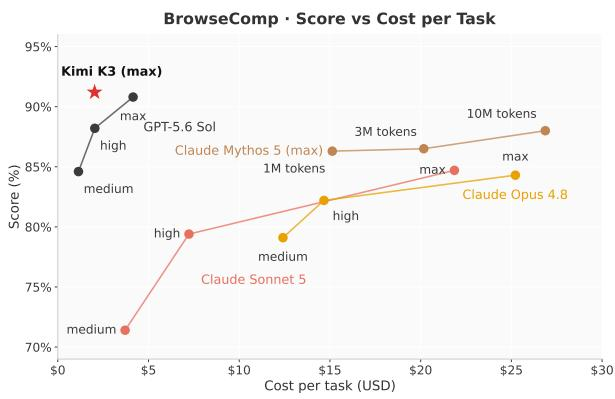
\includegraphics[keepaspectratio,alt={image}]{images/5388629fd9345d3dd3c6986ac771a2a56893862b20fb623a28246d3b2a4f6b5c.jpg}}

\begin{enumerate}
\def\labelenumi{(\alph{enumi})}
\setcounter{enumi}{1}
\tightlist
\item
  BrowseComp
\end{enumerate}

\pandocbounded{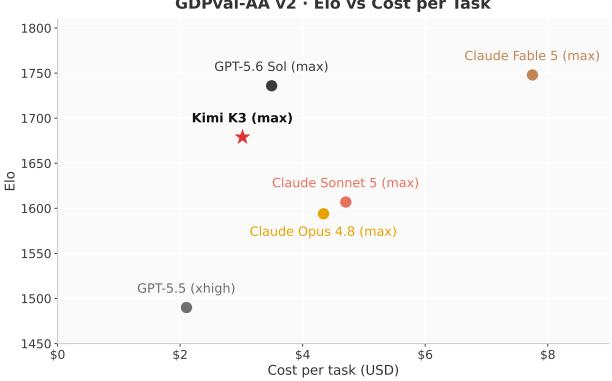
\includegraphics[keepaspectratio,alt={image}]{images/7c7188b3bd96c38d416cba3988a4c2ade19e7d50f6fd921c477852b340a0711d.jpg}}

\begin{enumerate}
\def\labelenumi{(\alph{enumi})}
\setcounter{enumi}{2}
\tightlist
\item
  GDPval-AA v2
\end{enumerate}

\pandocbounded{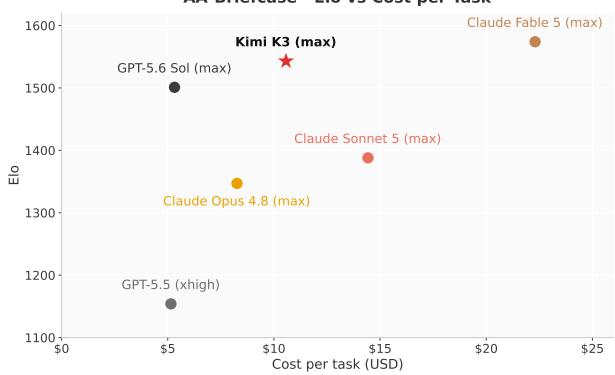
\includegraphics[keepaspectratio,alt={image}]{images/a9db98cdf558490a9d68f5a1174388fb4b4869bfd9ad23417894b1fda6b2be84.jpg}}

\begin{enumerate}
\def\labelenumi{(\alph{enumi})}
\setcounter{enumi}{3}
\tightlist
\item
  AA-Briefcase
\end{enumerate}

图 13: Kimi Code Bench 2.0、BrowseComp、GDPval-AA v2 和 AA-Briefcase
的得分与单任务推理成本对比。Kimi K3 以星号标记。

总体而言，Kimi K3 在所有四个套件中均位于或接近成本效率前沿，以远低于
Claude Fable 5 的成本提供接近顶尖的分数。
